\chapter{N-Grams y FSA}

\section{N-Grams}

\textit{``Hello, how are \dots''}\\
Dada secuencia de palabras $w_1, w_2, \ldots, w_n$, queriamos predecir la siguiente palabra $w_{n+1}$.
O, mejor, queriamos establecer la probabilid de una secuencia de palabras $P(w_1, w_2, \ldots, w_n)$, que se puede decomponer en
\begin{equation}
P(w_1, w_2, \ldots, w_n) = P(w_1) P(w_2|w_1) P(w_3|w_1, w_2) \ldots P(w_n|w_1, w_2, \ldots, w_{n-1})
\end{equation}


Objectives:
\begin{itemize}
	\item To assign a probability score to every word sequence
	\item To reflect a previous knowledge of a text source
   \begin{itemize}
	   \item To predict the most likely occurrence of words using its context
   \end{itemize}
\end{itemize}

\begin{equation}
   P(w) = P(w_1)\cdot \prod_{i=2}^{m}P(w_i|w_1, w_2, \ldots, w_{i-1}) \textit{ with } m \in \Sigma
\end{equation}

La estimación de la probabilidad $P(w)$ es prohibitivamente costoso cuando el tamaño del vocabulario $|\Sigma|$ 
se hace enorme: $|\Sigma|^{i-1}$ diferentes historias posibles.

Entonces, tal probabilidad se puede aproximar:
\begin{equation}
   P(w) \approx \prod_{i=2}^{m}P(w_i|\phi(w_1, w_2, \ldots, w_{i-1})) = \prod_{i=2}^{m}P(w_i|w_1, w_2, \ldots, w_{i-1})
\end{equation}

La estimación de la probabilidad típicamente se hace usando relative frequency counts $f(\cdot | \cdot)$:
\begin{equation}
   P(w_i|w_1, w_2, \ldots, w_{i-1}) = f(w_i|w_1, w_2, \ldots, w_{i-1}) =
   \frac{C(w_1, w_2, \ldots, w_i)}{C(w_1, w_2, \ldots, w_{i-1})}
\end{equation}

\begin{figure}[htbp]
   \centering
   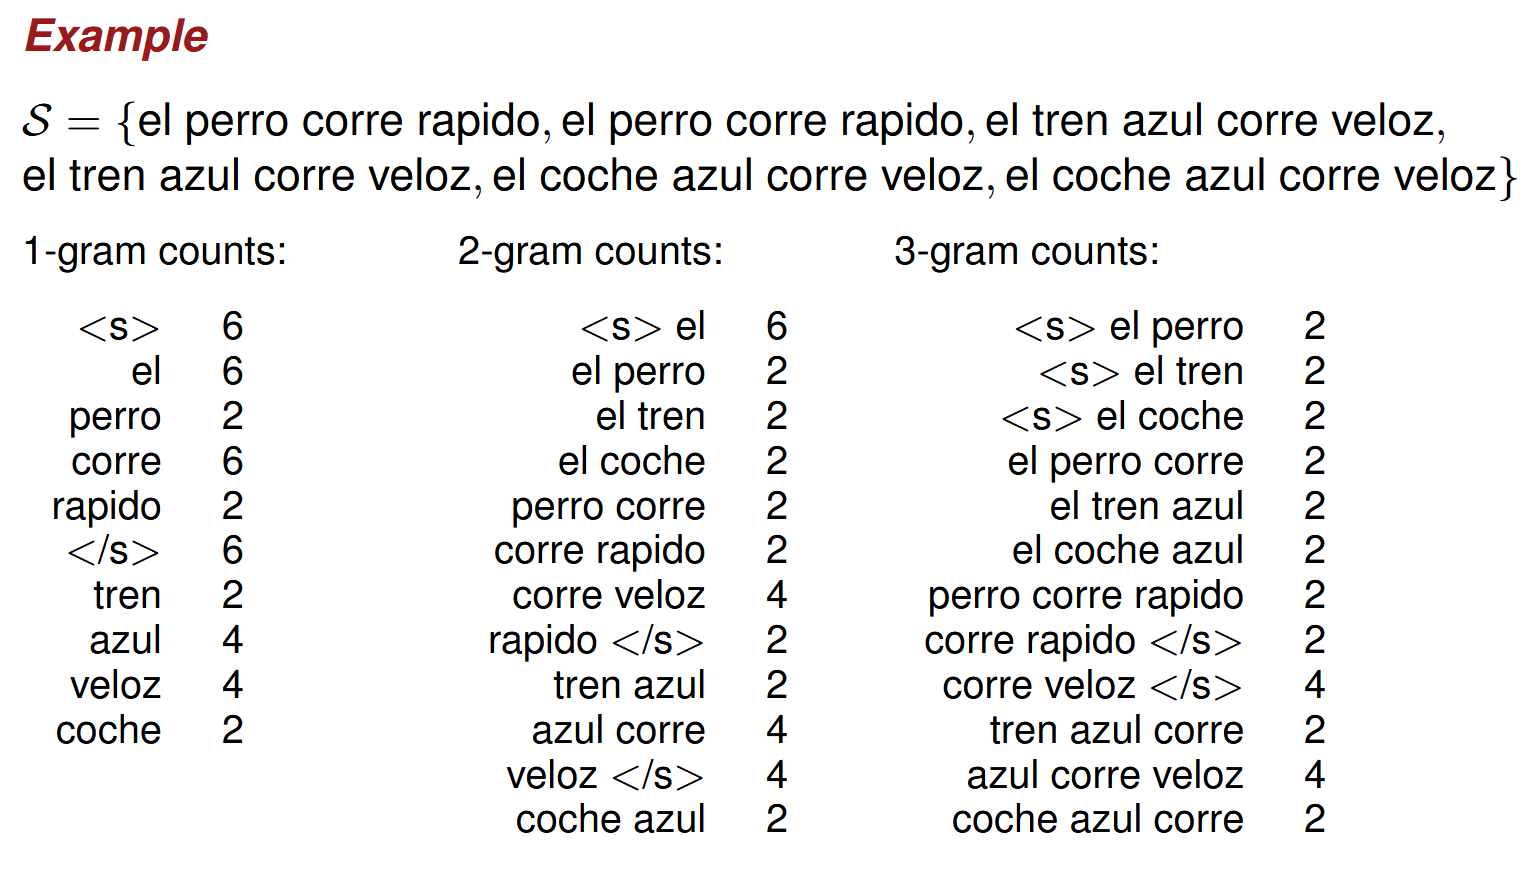
\includegraphics{images/07/ngramExample.png}
   \caption{N-Grams Example}
   \label{fig:07/ngramExample}
\end{figure}

Un LM (Language Model, o Modelo de Lenguaje) es un modelo probabilístico que asigna una probabilidad a una secuencia de palabras.
Un N-gram LM se dice \textit{completo} si todas las posibles secuencias de palabras tienen una apropiada estimación de probabilidad.\\
El problema con esto es que hay eventos (secuencias de palabras) que casi nunca ocurren en el corpus de entrenamiento (\textit{training set}), y por lo tanto no tienen una estimación de probabilidad.
Por este motivo hay métodos de \textit{smoothing} y \textit{discounting}.

\begin{table}[htbp]
   \centering
   \begin{tabular}{|c|c|}
      \hline
      \textbf{Smoothing} & \textbf{Discounting}\\
      \hline
      Back-Off & Good Turing\\
      Interpolation & Absolute Discounting\\
      & Witten Bell\\
      & Linear Discounting\\
      & Kneser-Ney\\
      & ...\\
      \hline
   \end{tabular}
   \caption{Smoothing and discounting}
   \label{tab:smoothingAndDiscounting}
\end{table}


\begin{figure}[htbp]
   \centering
   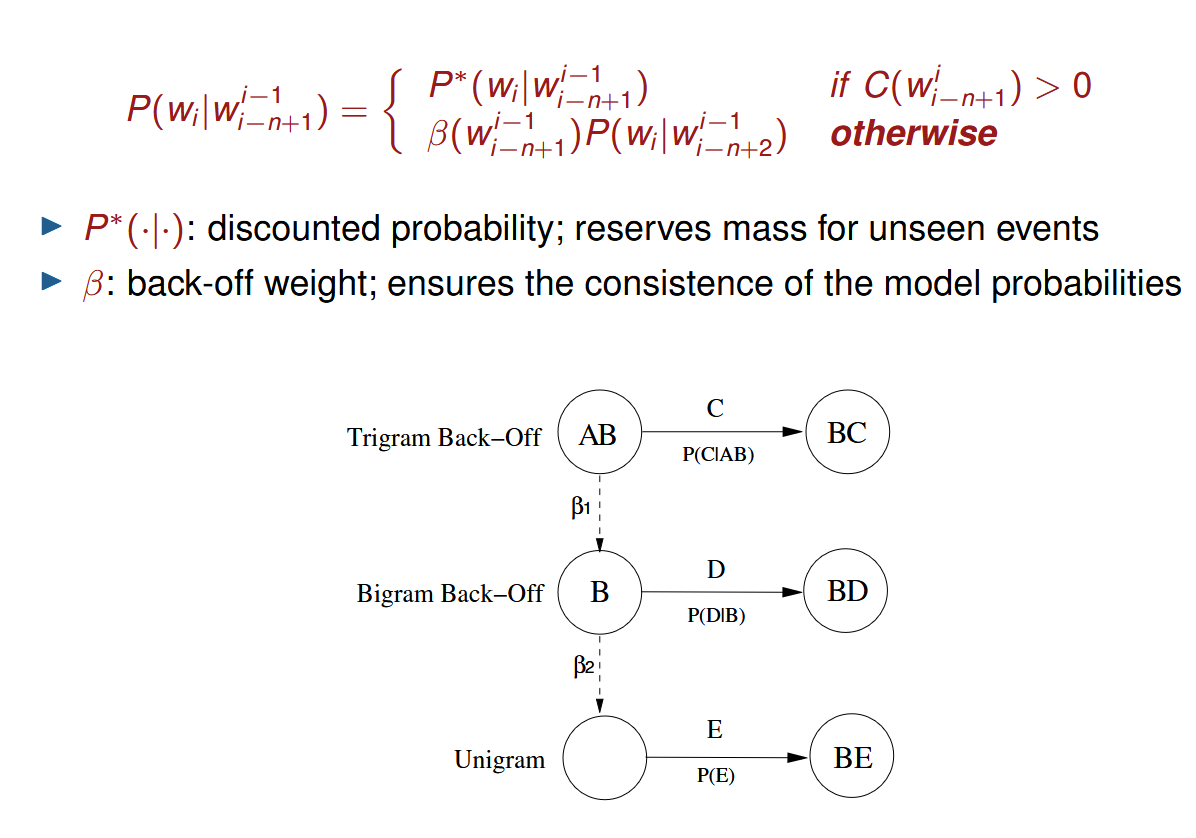
\includegraphics{images/07/ngramBackOff.png}
   \caption{07/ngramBackOff}
   \label{fig:07/ngramBackOff}
\end{figure}


\begin{verbatim}
   Ejercicio

   1-Gram
   P(<s>)	P(el)	P(perro)	P(corre)	P(rapido)	P(</s>)
   6        6     2        6        2	       6	        81
   -        -     -        -	       -        -    =    -     * 10^-6
   34       34    34       34	      34	      34		      64
   
   34 perché la somma delle occorrenze delle singole parole è 40, a cui però dobbiamo togliere 
   le 6 occorrenze della marca di fine stringa, perché quella non contribuisce ai possibili
    prefissi (historia)    

   
   2-GRAM
   P(<s>) 	P(el|<s>)	P(perro|el)	P(corre|perro)	P(rapido|corre)	P(</s>|rapido)
   0	6		2		2		2		2		  1
     -		-		-		-		-		= -		
     6		6		2		6		2		  9
   
   3-GRAM
   
   P(<s>)	P(el|<s>)	P(perro|<s>el)	P(corre|el perro)	P(rapido|perro corre)	P(</s>|corre rapido)
   0	0		2		1			1			1
         6

\end{verbatim}

\section{FSA - Finite State Automata}
Introduction to PFA
Introduction to Probabilistic Finite-State Automata
\begin{itemize}
   \item Free Monoid $\Sigma^*$: Given a finite set $\Sigma$, $\Sigma^+$ is the set of all strings with finite length composed of elements from $\Sigma$
   \begin{equation}
      \Sigma^* = \Sigma^+ \cup \{\lambda\} \text{($\lambda$ is the empty string)}
   \end{equation}
   \item Grammar: $G = (N, \Sigma, R, S)$
\end{itemize}
\begin{itemize}
   \item $N$: Finite set of non-terminal symbols
   \item $\Sigma$: Finite set of terminal symbols or primitives
   \item $S \in N$: Initial non-terminal symbol or ``axiom"
   \item $R \subset (N \cup \Sigma)^*N(N \cup \Sigma)^* \times (N \cup \Sigma)^*$: set of rules
\end{itemize} or productions
A rule is written as:
\begin{equation}
   \alpha \rightarrow \beta,\quad \alpha \in (N \cup \Sigma)^*N(N \cup \Sigma)^*, \quad \beta \in (N \cup \Sigma)^*
\end{equation}

\paragraph*{Elemental derivation: $\Rightarrow G$:}
$\mu \alpha \delta \Rightarrow_G \mu \beta \delta \iff \exists(\alpha \rightarrow \beta) \in R, \mu, \delta \in (N \cup \Sigma)^*$

\paragraph*{Derivation $\stackrel{*}{\Rightarrow}_G$:}
It is a finite sequence of elemental derivations.
A derivation $d$ can be written as the corresponding rule sequence of $G$.
The set of derivations of $y \in \Sigma^*$ (such that $S \stackrel{*}{\Rightarrow}_G y$) is written as $D_G(y)$.
A grammar $G$ is ambiguous if $\exists y \in \Sigma^*$ such that $|D_G(y)| > 1$.

\framedt{Derivation}{
Quindi:\\
    $\alpha$ è la parte sinistra della regola, chiamata anche contesto o parte da sostituire. È una stringa che deve contenere almeno un non terminale, poiché solo i non terminali possono essere sostituiti.

    $\beta$ è la parte destra, cioè ciò che sostituisce $\alpha$ durante la derivazione.

Supponiamo:
\begin{align*}
   N={A,B}\\
   \Sigma={a,b}\\
   R={aAb\rightarrow abb}\\
   \alpha=aAb\\
   \beta=abb
\end{align*}

La regola dice che se in una stringa troviamo la sottostringa $aAb$, possiamo sostituirla con $abb$.

L'elemento:
\begin{align*}
   \mu\alpha\sigma\Rightarrow_{G}\mu\beta\sigma
\end{align*}

significa che:\\
    Se in una stringa $\mu\alpha\sigma$, si trova la sottostringa $\alpha$,
    E se esiste una regola $\alpha\rightarrow\beta\in R$,
    Allora si può sostituire $\alpha$ con $\beta$, ottenendo $\mu\beta\sigma$.

Quindi, $\alpha$ e $\beta$ sono le parti centrali della riscrittura, mentre $\mu$ e $\sigma$ rappresentano il contesto a sinistra e a destra, rispettivamente.
}

\paragraph*{Language generated by a grammar $G$, $L(G)$:}
$L(G) = \{y \in \Sigma^* \mid S \stackrel{*}{\Rightarrow}_G y\}$

\begin{itemize}
	\item \textbf{Regular grammars}: $G = (N, \Sigma, R, S)$,
Rules of $R: A \rightarrow aB \vee A \rightarrow a, A, B \in N, a \in \Sigma$
	\item \textbf{Finite-state automaton}: (non deterministic)

   \begin{equation*}
      A = (Q, \Sigma, \delta, q_0, F ),\quad q_0 \in Q,\quad F \subseteq Q,\quad \delta : Q \times \Sigma \rightarrow 2^Q
   \end{equation*}
	\item \textbf{Equivalence}: For each regular grammar there exists a finite-state automaton that recognizes the same language\footnote{The contrary isn't always true for stachastic languages.}
\end{itemize}

\begin{figure}[htbp]
   \centering
   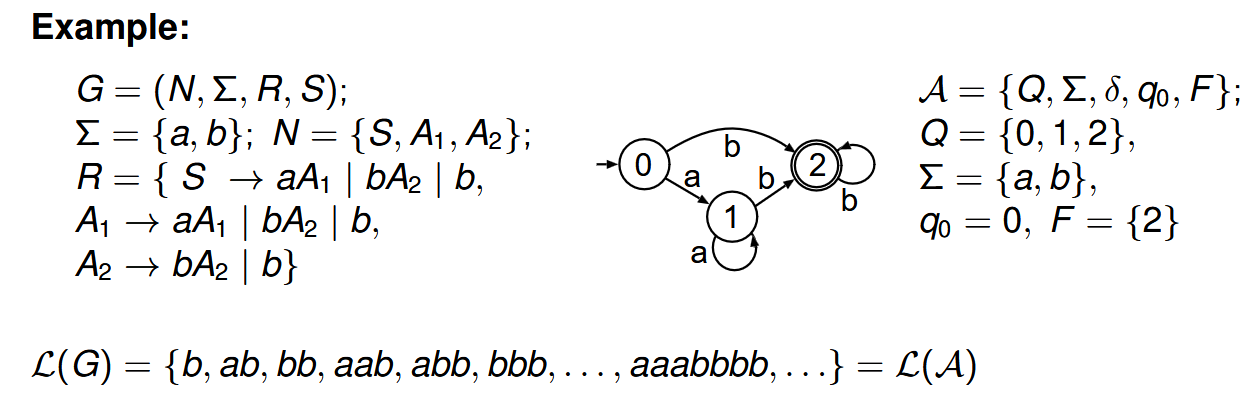
\includegraphics{images/07/fsaEquivalence.png}
   \caption{FSA Equivalence example}
   \label{fig:07/fsaEquivalence}
\end{figure}

Probabilistic Finite-state Automata (PFA): it is a tuple
$A = \langle Q, \Sigma, \delta, I, F , P\rangle $, where:


\begin{itemize}
   \item $Q$: finite set of states
   \item $\Sigma$: finite alphabet of symbols
   \item $\delta \subseteq Q \times \Sigma \times Q$: transition function
   \item $I: Q \rightarrow \mathbb{R}^+ \cup \{0\}$: initial state probabilities, with $\sum_{q \in Q} I(q) = 1$
   \item $F: Q \rightarrow \mathbb{R}^+ \cup \{0\}$: final state probabilities
   \item $P: \delta \rightarrow \mathbb{R}^+ \cup \{0\}$: transition probabilities,  such that
   \begin{equation}
      \text{with } \forall q \in Q: F(q) + \sum_{q' \in Q, \sigma \in \Sigma} P(q,\sigma,q') = 1
   \end{equation}
\end{itemize}

A path in a PFA is a sequence of transitions: $\pi = (q_0, a_1, q_1)(q_1, a_2, q_2)...(q_{n-1}, a_n, q_n)$

The probability of a path $\pi$ is:
\begin{equation}
P(\pi) = I(q_0) \cdot \left(\prod_{i=1}^{n} P(q_{i-1}, a_i, q_i)\right) \cdot F(q_n)
\end{equation}

The probability of a string $x = a_1a_2...a_n$ is the sum of probabilities of all paths that generate $x$:
\begin{equation}
P_A(x) = \sum_{\pi \in \Pi_A(x)} P(\pi)
\end{equation}
where $\Pi_A(x)$ is the set of all paths in automaton $A$ that generate string $x$.

\begin{figure}[htbp]
   \centering
   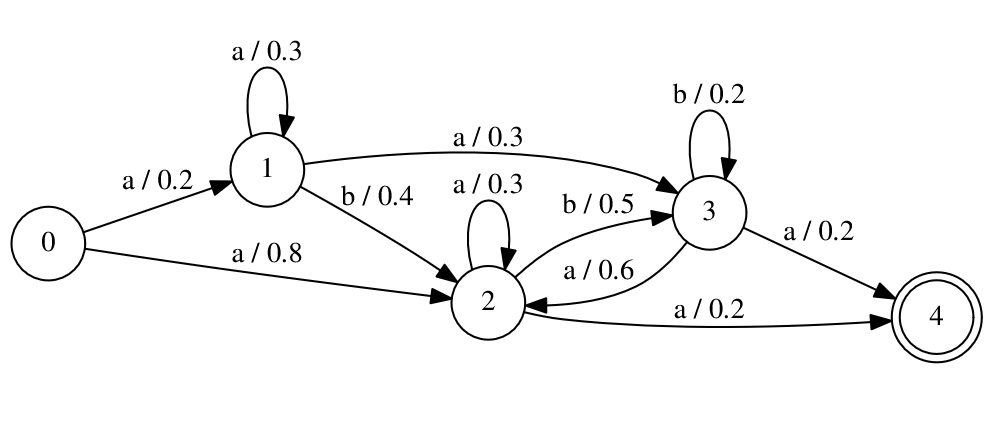
\includegraphics{images/07/pfaExample.png}
   \caption{Example of a Probabilistic Finite-state Automaton}
   \label{fig:07/pfaExample}
\end{figure}

\subsection{Applications of PFA}

PFAs are widely used in:
\begin{itemize}
   \item Speech recognition
   \item Natural language processing
   \item Pattern recognition
   \item Biological sequence analysis
\end{itemize}

\subsection{Relation between N-Grams and PFA}

Any n-gram model can be represented as a PFA, where:
\begin{itemize}
   \item States represent histories (previous n-1 words)
   \item Transitions represent word emissions with their corresponding probabilities
   \item The resulting automaton has a specific structure reflecting the Markov property of n-gram models
\end{itemize}

% // TODO tres transparencias

\section{Relación entre N-Grams y PFA}

\begin{figure}[htbp]
   \centering
   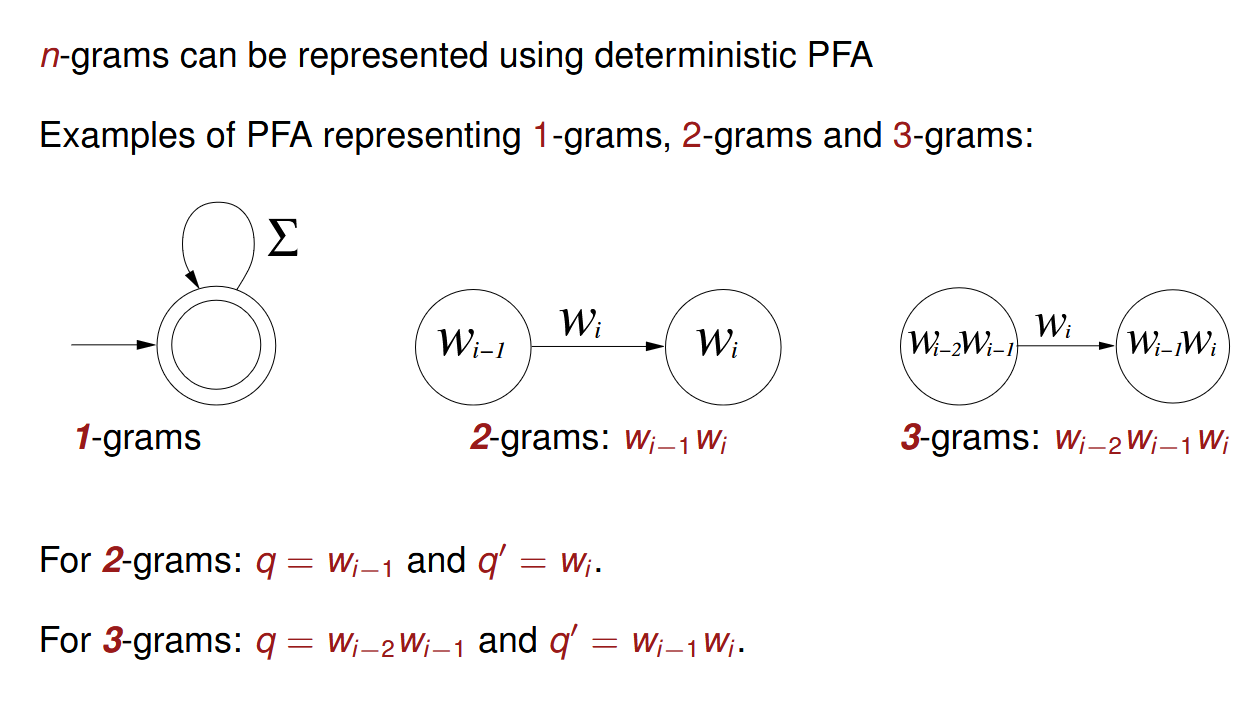
\includegraphics{images/07/ngramFSA.png}
   \caption{N-Gram representados como FSA}
   \label{fig:07/ngramFSA}
\end{figure}


